\documentclass[11pt]{article}
\usepackage[margin=1in]{geometry}
\usepackage{graphicx}
\usepackage{booktabs}
\usepackage{xcolor}
\usepackage{hyperref}
\usepackage{amsmath}
\usepackage{listings}
\usepackage{enumitem}
\usepackage{caption}
\usepackage{float}
\usepackage{longtable}

\hypersetup{colorlinks=true, linkcolor=blue, urlcolor=blue, citecolor=blue}

\definecolor{codebg}{rgb}{0.96,0.96,0.96}
\lstset{
  basicstyle=\ttfamily\small,
  backgroundcolor=\color{codebg},
  frame=single,
  breaklines=true,
  columns=fullflexible,
  keywordstyle=\color{blue!70!black}\bfseries,
  commentstyle=\color{green!40!black}\itshape,
  stringstyle=\color{orange!70!black},
  language=C++,
  tabsize=2,
}

\title{\Large\textbf{Lab Assignment Report: Flow Control Mechanisms\\ of the Data Link Layer}}
\author{Sajjad Ahmed Shaaz \\ 002410501093 \\ BCSE-III A3}
\date{September 21, 2026}

\begin{document}
\maketitle

\section*{Basic Information}
\begin{itemize}[leftmargin=1.6em]
  \item \textbf{Subject:} CSE/PC/B/S/314 Computer Networks Lab
  \item \textbf{Assignment Number:} 2
  \item \textbf{Problem Statement:} Design and implement flow control mechanisms of the
  Logical Link Control sub-layer of the Data Link Layer within a simulated network
  environment: Stop-and-Wait ARQ, Go-Back-N ARQ, and Selective Repeat ARQ, each built on
  the Framing/Channel/Send/Timer/Timeout/Recv method set specified in the assignment, and
  reusing the CRC/Checksum and error-injection modules from Assignment 1.
  \item \textbf{Code demonstration due:} 24--28 August 2026 \quad
  \textbf{Report submission due:} 31 August -- 4 September 2026
\end{itemize}

\section{Design}

\subsection{Purpose of the Program}
Assignment 1 verified that a receiver can \emph{detect} a corrupted frame. This assignment
answers the next question: once a frame is known to be lost, corrupted, or arrives out of
order, how does the sender recover it without the two endpoints losing synchronization, and
how much throughput does that recovery cost? Three flow-control disciplines are implemented
end-to-end over a simulated lossy/delaying/corrupting channel — Stop-and-Wait, Go-Back-N
ARQ, and Selective Repeat ARQ — and compared under identical, reproducible channel
conditions so that their textbook trade-offs (idle time, retransmission cost, buffering
requirements) can be measured rather than only asserted.

\subsection{Design Rationale}
All three protocols are built on one shared library (\texttt{common/}) so that framing, the
FCS module, error injection, and the channel simulation cannot silently differ between
protocols — any measured difference in the results is therefore attributable to the flow-control
logic itself, not to incidental implementation drift. Each protocol pair is two independent
OS processes (sender, receiver) communicating over \textbf{UDP} on loopback: UDP is
message-oriented, so one datagram maps cleanly to one frame, and — critically for this
assignment — UDP does not itself retransmit or reorder, so any reliability the transfer
exhibits is entirely a property of the ARQ logic being tested, not of the transport.

A single \texttt{Channel()} routine (\texttt{common/channel.cpp}) is reused by \emph{both}
directions: the sender passes every outgoing data frame through it, and the receiver passes
every outgoing ACK through it, each with its own independently configurable loss and
bit-error probability. This lets the test harness satisfy the assignment's requirement to
vary ``probability of an error or delay in the transmission of a packet \emph{or in its
acknowledgment}'' without special-casing either direction.

\subsection{Frame Format}
Figure~\ref{fig:dataframe} and Figure~\ref{fig:ackframe} show the two frame types to scale.
The Data Frame header follows Fig.~1 of the assignment (source/destination MAC, length,
sequence number); the sequence field is 1 byte, so it wraps modulo 256 — Go-Back-N is
therefore bounded to $N \le 255$ and Selective Repeat to the standard $N \le 128$ bound
(half the sequence space), enforced in code so a wrapped sequence number can never be
ambiguous within one window. The FCS trailer's width is scheme-dependent (1--4 bytes,
Assignment 1's five schemes are all available); CRC-32 (4 bytes) is used as the default
to match the frame size shown in the assignment's Fig.~1.

\begin{table}[H]
\centering
\begin{tabular}{llp{7cm}}
\toprule
\textbf{Field} & \textbf{Size} & \textbf{Purpose} \\
\midrule
Source MAC & 6 bytes & Sender hardware address \\
Destination MAC & 6 bytes & Receiver hardware address \\
Length & 2 bytes & Original (unpadded) payload length \\
Sequence number & 1 byte & Per-frame index, wraps mod 256 \\
Payload & 46 bytes & Data chunk (zero-padded if short) \\
FCS & 1--4 bytes & Checksum-16 / CRC remainder (4 bytes for the default, CRC-32) \\
\bottomrule
\end{tabular}
\caption{Data Frame header layout (Fig.~1 of the assignment).}
\end{table}

\begin{figure}[H]
\centering
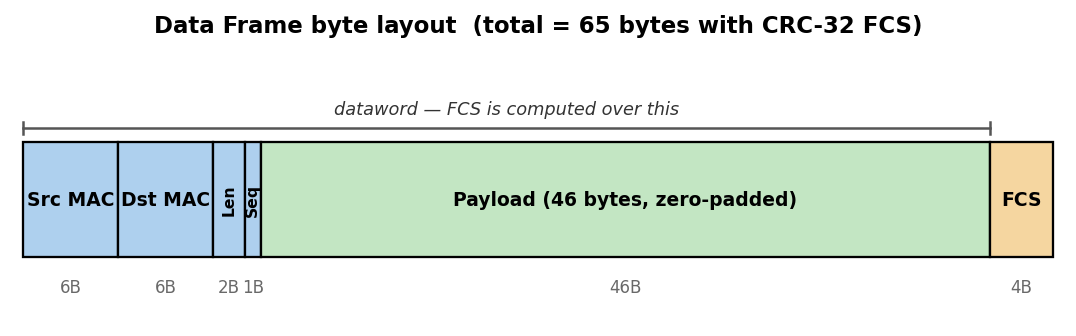
\includegraphics[width=\textwidth]{figures/data_frame_layout.png}
\caption{Data Frame byte layout drawn to scale. The dataword (everything but the FCS) is
what the check sequence is computed over.}
\label{fig:dataframe}
\end{figure}

\begin{figure}[H]
\centering
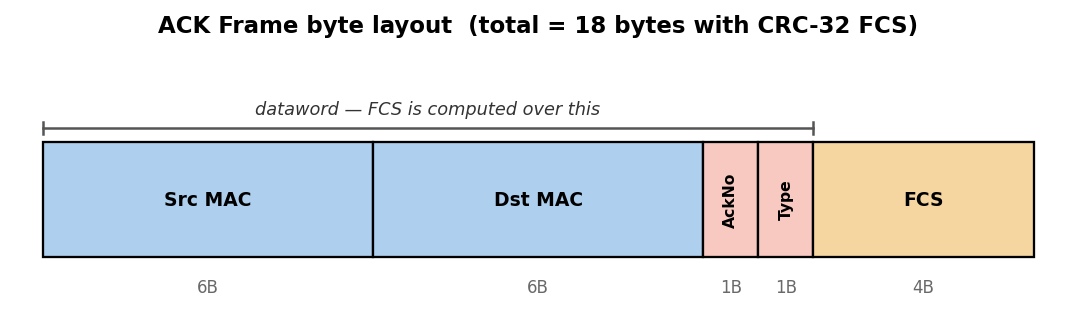
\includegraphics[width=\textwidth]{figures/ack_frame_layout.png}
\caption{ACK Frame byte layout. \texttt{AckNo} carries the acknowledged sequence number
(cumulative for Stop-and-Wait/Go-Back-N, independent per-frame for Selective Repeat);
\texttt{Type} is reserved (0 = ACK).}
\label{fig:ackframe}
\end{figure}

\subsection{Structure Diagram (Procedural Organization)}
Figure~\ref{fig:arch} shows the shared procedural structure that all three protocols
instantiate. The sender's \texttt{Send()} decides whether to transmit a new frame or
retransmit an outstanding one; \texttt{Timer()}/\texttt{Timeout()} maintain an adaptive
round-trip estimate that governs when a retransmission is triggered; \texttt{Recv()}
validates an incoming ACK and slides the send window. The receiver's \texttt{Recv()} parses
an incoming datagram, \texttt{Check()} recomputes and compares the FCS, and the frame is
then accepted (delivered, and for Selective Repeat possibly buffered out of order) or
discarded before an ACK is built and sent back through the same simulated channel.

\begin{figure}[H]
\centering
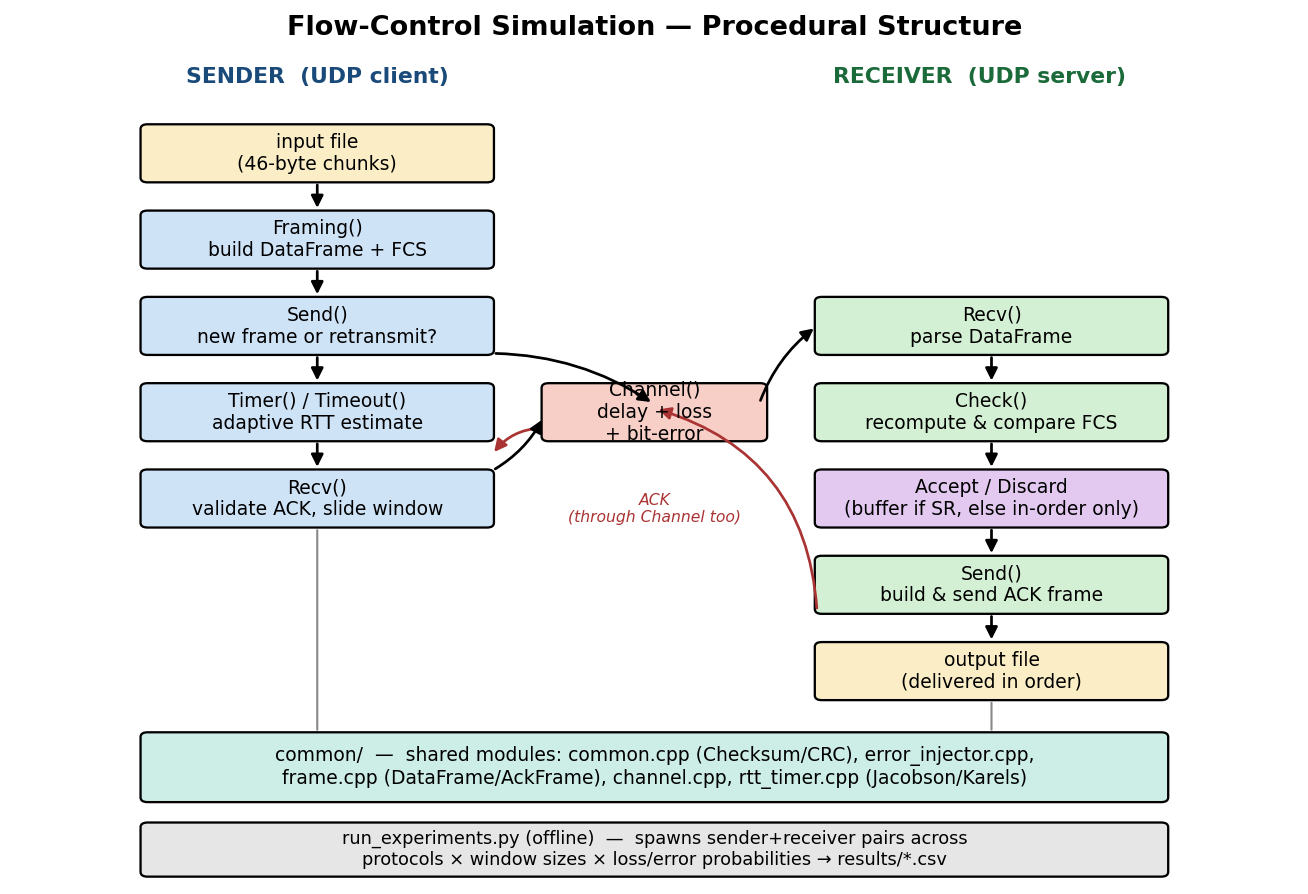
\includegraphics[width=\textwidth]{figures/architecture.png}
\caption{Procedural structure shared by all three flow-control protocols.}
\label{fig:arch}
\end{figure}

\subsection{Input and Output Format}
\textbf{Input:} a text file passed on the sender's command line, together with the window
size $N$ (Go-Back-N/Selective Repeat only), the data-channel loss and bit-error
probabilities, and the FCS scheme. \textbf{Output:} the receiver reconstructs the file
byte-for-byte at the path given on its own command line; both endpoints additionally print a
human-readable run summary to \texttt{stderr} and the sender prints one \texttt{RESULT,...}
CSV line to \texttt{stdout} (protocol, window, loss/error probability, frame counts,
retransmissions, elapsed time, average RTT, throughput, efficiency) that the automated test
harness (\texttt{run\_experiments.py}) collects into \texttt{results/*.csv}.

\section{Implementation}
The project is implemented in C++17, POSIX sockets, split into a shared library and three
protocol-specific sender/receiver pairs.

\subsection{Component Breakdown}
\begin{itemize}[leftmargin=1.6em]
  \item \texttt{common/common.h/.cpp} --- the five FCS calculators, ported unchanged from
  Assignment 1.
  \item \texttt{common/error\_injector.h/.cpp} --- bit-flip corruption (single / two-isolated
  / odd / burst), also ported from Assignment 1.
  \item \texttt{common/frame.h/.cpp} --- \texttt{DataFrame} and \texttt{AckFrame}
  (de)serialization and FCS verification; \texttt{framing()} chunks an input file into a
  \texttt{vector<DataFrame>}.
  \item \texttt{common/channel.h/.cpp} --- the simulated wire: a random 1--15\,ms
  propagation delay is always applied, then a \texttt{lossProb} roll silently drops the
  frame (never sent — models both loss and an unbounded delay that forces a timeout), else
  an \texttt{errorProb} roll flips a bit before sending.
  \item \texttt{common/rtt\_timer.h/.cpp} --- the adaptive retransmission timer
  (\texttt{Timer()}/\texttt{Timeout()}), Jacobson/Karels estimation as used by TCP.
  \item \texttt{common/socket\_util.h} --- socket setup, one port pair per protocol, and the
  one-shot \texttt{SETUP} bootstrap handshake.
  \item \texttt{stop\_and\_wait/}, \texttt{go\_back\_n/}, \texttt{selective\_repeat/} ---
  \texttt{sender.cpp} / \texttt{receiver.cpp} for each protocol.
  \item \texttt{run\_experiments.py} --- spawns sender/receiver subprocess pairs across
  protocols $\times$ window sizes $\times$ loss/error probabilities, diffs the delivered file
  against the original, and aggregates \texttt{results/*.csv}.
\end{itemize}

\subsection{Adaptive Timer: \texttt{Timer()} / \texttt{Timeout()}}
Each sender maintains one Jacobson/Karels estimator (\texttt{RttTimer}):
\[
\text{EstimatedRTT} \leftarrow (1-\alpha)\,\text{EstimatedRTT} + \alpha\,\text{SampleRTT},
\qquad
\text{DevRTT} \leftarrow (1-\beta)\,\text{DevRTT} + \beta\,|\text{SampleRTT} - \text{EstimatedRTT}|
\]
\[
\text{Timeout} = \text{EstimatedRTT} + 4 \cdot \text{DevRTT}, \qquad \alpha = 0.125,\ \beta = 0.25
\]
\texttt{onSample()} implements \texttt{Timeout()}: every clean round trip folds a fresh RTT
sample into the estimate and recomputes the timeout used for the \emph{next} transmission.
Critically, only frames that were \textbf{not} retransmitted feed a sample (Karn's
algorithm) — an ACK arriving after a retransmission is ambiguous (it could belong to the
original send or the retransmission), so sampling it would corrupt the estimator with a
stale delay.
\begin{lstlisting}
void RttTimer::onSample(double sampleRttMs) {
    devRtt_ = (1 - BETA) * devRtt_ + BETA * std::abs(sampleRttMs - estRtt_);
    estRtt_ = (1 - ALPHA) * estRtt_ + ALPHA * sampleRttMs;
    timeout_ = estRtt_ + 4 * devRtt_;
}
\end{lstlisting}

\subsection{Stop-and-Wait ARQ}
Window size is fixed at 1 on both ends. The sender sends one frame and blocks until either
a matching ACK or a timeout occurs; on timeout \emph{or} a corrupted/mismatched ACK it
resends the identical frame. The receiver tracks a single \texttt{expected} sequence
counter: a frame equal to \texttt{expected} is delivered and ACKed; a frame equal to the
\emph{previous} accepted sequence is a duplicate (its ACK was lost) and only its ACK is
re-sent; a frame that fails FCS is silently discarded, which is what forces the sender's
timeout.
\begin{lstlisting}
while (!acked) {
    channelSend(fd, f.toBytes(), dst, cfg, chStats);           // Send()
    setRecvTimeoutMs(fd, timer.timeoutMs());                   // Timer()
    ssize_t n = recvfrom(fd, buf, sizeof(buf), 0, ...);         // Recv()
    if (n == ackFrameSize && ackValid && a.ackno == f.seq) {
        acked = true;
        if (!isRetransmission) timer.onSample(rttMs);           // Timeout()
    } else {
        isRetransmission = true;                                // retransmit same frame
    }
}
\end{lstlisting}

\subsection{Go-Back-N ARQ}
The sender keeps a window \texttt{[base, nextSeq)} of at most $N$ outstanding frames but a
\textbf{single shared timer} for the whole window. A cumulative ACK for sequence $S$
advances \texttt{base} past every frame up to and including $S$; on timeout (or a garbled
ACK) the \emph{entire} outstanding window is retransmitted — the defining ``go back $N$''
cost. The receiver has window size 1: it accepts only the exact next in-order frame,
discards anything corrupted or out of order (no buffering), and — as a practical
optimization common in textbook implementations — re-sends its last cumulative ACK on an
out-of-order arrival so a lost ACK need not always wait for a full window timeout.
\begin{lstlisting}
while (base < total) {
    while (nextSeq < total && nextSeq < base + windowN)         // fill window
        { channelSend(...); nextSeq++; }
    ssize_t n = recvfrom(...);                                   // wait once for the window
    if (validCumulativeAck)
        base = index_of(ackno) + 1;                              // slide past acked run
    else
        for (i = base; i < nextSeq; i++) channelSend(frames[i]); // go back N: resend window
}
\end{lstlisting}

\subsection{Selective Repeat ARQ}
Both windows are size $N$. The sender gives every outstanding frame its \emph{own}
deadline, ACKs are non-cumulative (one frame acknowledged at a time), and only the
individual frame(s) whose personal deadline has elapsed are resent — never the whole
window. The receiver buffers any correctly received frame even if out of order, ACKs every
accepted frame individually, discards only corrupted frames, and flushes the contiguous run
starting at its delivery cursor to the output file as soon as it becomes available; a frame
mapping to an index behind the delivery cursor is a duplicate (its original ACK was lost)
and is re-ACKed without touching the buffer.
\begin{lstlisting}
// sender: resend only frames whose OWN deadline has passed
for (int i = base; i < nextSeq; i++)
    if (!acked[i] && now >= deadline[i]) sendFrame(i, now);

// receiver: deliver the contiguous run, buffer holes
while (deliverIdx < total && got[deliverIdx])
    { out.write(buf[deliverIdx].payload...); deliverIdx++; }
\end{lstlisting}
Figure~\ref{fig:timeline} contrasts what is outstanding at once and how a loss is recovered
in each scheme; note that Go-Back-N discards frames D4--D6 that arrive after a gap and must
resend the whole window, whereas Selective Repeat resends only the single lost frame D1 and
keeps everything else it already buffered.

\begin{figure}[H]
\centering
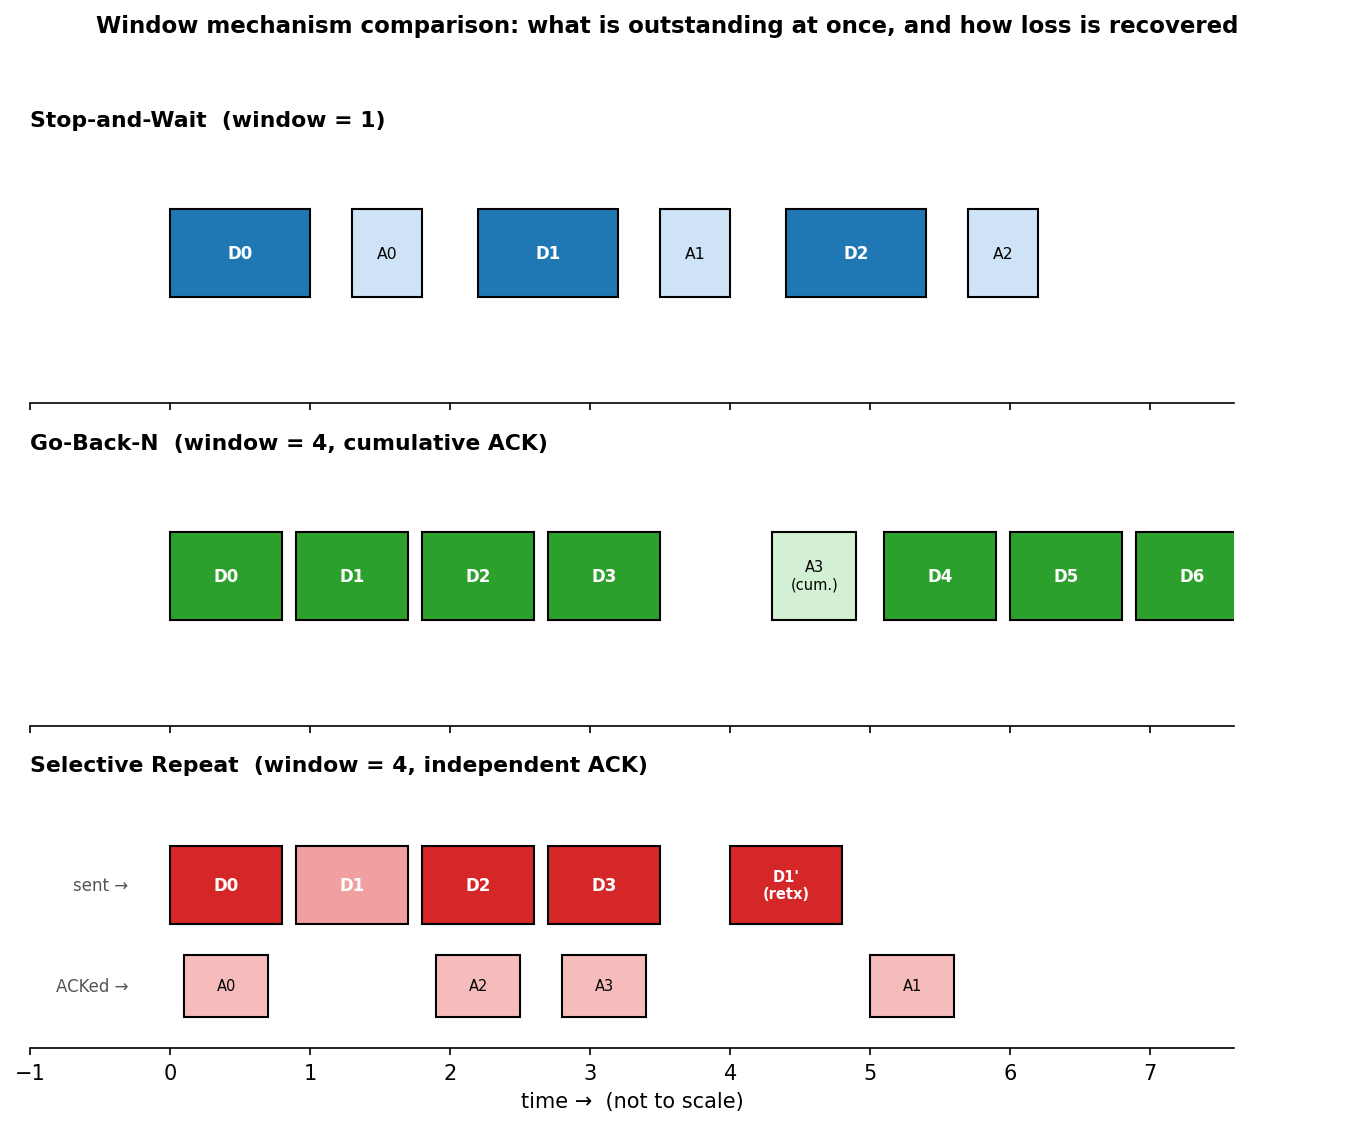
\includegraphics[width=\textwidth]{figures/window_timeline.png}
\caption{Window mechanism comparison across the three protocols.}
\label{fig:timeline}
\end{figure}

\subsection{Performance Metrics}
The sender computes three metrics per run:
\begin{itemize}[leftmargin=1.6em]
  \item \textbf{Average RTT} --- wall-clock time from send to a matching ACK, sampled
  \emph{only} for frames that succeeded on their first attempt (Karn's rule, \S2.2). This
  isolates pure round-trip time from retransmission-induced delay, and is what answers the
  assignment's ``compare time between the propagation of a packet and reception of its
  ACK.''
  \item \textbf{Throughput} $= \dfrac{\text{file size (bytes)}}{\text{elapsed wall-clock
  time}}$ --- the whole transfer, including every timeout and retransmission.
  \item \textbf{Efficiency} $= \dfrac{\text{unique frames in the file}}{\text{total frame
  transmissions attempted}} \times 100\%$ --- since frame size is constant within a run,
  this ratio is identical to (useful bytes delivered)/(total bytes put on the wire); it
  isolates how much of the sender's effort was ``wasted'' on retransmission, independent of
  how long that effort took.
\end{itemize}

\section{Test Cases}
Correctness was verified functionally (the receiver's output file must be byte-identical to
the sender's input file, checked with \texttt{diff} after every run) rather than only by
inspecting logs, across the following cases.

\begin{itemize}[leftmargin=1.6em]
  \item \textbf{TC1 --- Clean-channel correctness (all three protocols):} loss = error =
  0, a 730-frame (33{,}566-byte) input file. \emph{Checking:} the receiver's output is
  byte-identical to the input and efficiency is exactly 100\%.
  \item \textbf{TC2 --- Data-frame loss forces a timeout:} \texttt{lossProb} $>0$ on the
  data channel with a single frame outstanding (Stop-and-Wait). \emph{Checking:} the
  sender's \texttt{avg\_rtt\_ms} stays flat (Karn's rule excludes the retransmitted sample)
  while \texttt{elapsed\_ms} and \texttt{retransmissions} rise.
  \item \textbf{TC3 --- ACK loss / corruption:} \texttt{lossProb}/\texttt{errorProb} $>0$ on
  the ACK channel only. \emph{Checking:} the receiver's duplicate-detection path fires (it
  re-sends the stored ACK instead of re-delivering the payload) and the file is still
  reconstructed exactly once, in order.
  \item \textbf{TC4 --- Corrupted data frame is silently discarded:} \texttt{errorProb}
  $>0$ on the data channel. \emph{Checking:} \texttt{Check()} rejects the frame, no ACK is
  sent for it, and the sender's timeout (not an explicit NAK) is what triggers recovery.
  \item \textbf{TC5 --- Out-of-order handling differs by protocol:} force a gap by
  dropping one frame inside a window $N>1$. \emph{Checking:} Go-Back-N discards every frame
  behind the gap and retransmits the whole window; Selective Repeat buffers everything
  behind the gap and, once the lost frame is resent, delivers the buffered run in one flush
  without re-transmitting the frames the receiver already had.
  \item \textbf{TC6 --- Window-size sweep (Go-Back-N / Selective Repeat), clean channel:}
  $N \in \{1,2,4,8,16\}$ on the 730-frame file. \emph{Checking:} throughput increases with
  $N$; correctness (byte-identical output) holds at every $N$.
  \item \textbf{TC7 --- Impairment-probability sweep (all three protocols):} combined
  loss+error probability $p \in \{0, 0.1, 0.2, 0.3, 0.4, 0.5\}$ (split evenly,
  $\text{lossProb} = \text{errorProb} = p/2$, applied to both channels) on a 66-frame file,
  $N=4$ for the windowed protocols. \emph{Checking:} efficiency degrades monotonically with
  $p$ for every protocol and the file is still reconstructed correctly at every point,
  including $p=0.5$.
  \item \textbf{TC8 --- Selective Repeat duplicate/late-ACK handling:} a frame whose index
  falls behind the receiver's current delivery cursor (a retransmission whose original copy
  was already delivered because only its ACK was lost). \emph{Checking:}
  \texttt{resolveIndex()} maps it into the ``previous window'' range, the receiver re-ACKs
  it without touching the delivery buffer, and no duplicate bytes are written to the output
  file.
  \item \textbf{TC9 --- Malformed-datagram robustness:} an early implementation crashed
  with \texttt{std::out\_of\_range} when a duplicate 8-byte \texttt{SETUP} datagram was
  misparsed as a 65-byte data frame (found during testing, \S5.3). \emph{Checking:} every
  receive path now checks the datagram size against the exact expected frame size before
  parsing; stray/malformed datagrams are silently ignored instead of crashing.
\end{itemize}

All 29 configurations used for the Results section below (11 in Experiment A, 18 in
Experiment B) additionally exercise TC1/TC6/TC7 end-to-end and every one passed the
byte-identical \texttt{diff} check.

\section{Results}

\subsection{Experiment A --- Window Size Effect, Clean Channel}
A 730-frame (33{,}566-byte) file was transferred with \texttt{loss = error = 0},
Stop-and-Wait fixed at $N=1$, Go-Back-N and Selective Repeat swept across
$N \in \{1,2,4,8,16\}$. This isolates the throughput gain from pipelining alone.

\begin{table}[H]
\centering
\small
\begin{tabular}{lrrrrr}
\toprule
\textbf{Protocol} & \textbf{N} & \textbf{Elapsed (ms)} & \textbf{Avg RTT (ms)} & \textbf{Throughput (B/s)} & \textbf{Efficiency (\%)} \\
\midrule
Stop-and-Wait     & 1  & 12638.46 & 17.31  & 2655.86 & 100.00 \\
\midrule
Go-Back-N         & 1  & 12113.25 & 8.52   & 2771.02 & 100.00 \\
Go-Back-N         & 2  & 7779.24  & 13.38  & 4314.82 & 100.00 \\
Go-Back-N         & 4  & 6674.54  & 28.12  & 5028.96 & 100.00 \\
Go-Back-N         & 8  & 6470.22  & 61.93  & 5187.77 & 100.00 \\
Go-Back-N         & 16 & 6066.16  & 122.49 & 5533.32 & 100.00 \\
\midrule
Selective Repeat  & 1  & 12041.07 & 16.48  & 2787.63 & 100.00 \\
Selective Repeat  & 2  & 7788.87  & 21.32  & 4309.48 & 100.00 \\
Selective Repeat  & 4  & 6629.61  & 36.24  & 5063.04 & 100.00 \\
Selective Repeat  & 8  & 6488.76  & 68.22  & 5172.95 & 96.31 \\
Selective Repeat  & 16 & 7356.69  & 140.51 & 4562.65 & 87.64 \\
\bottomrule
\end{tabular}
\caption{Experiment A: window-size effect on a clean channel, 730 frames, CRC-32.}
\label{tab:expA}
\end{table}

\begin{figure}[H]
\centering
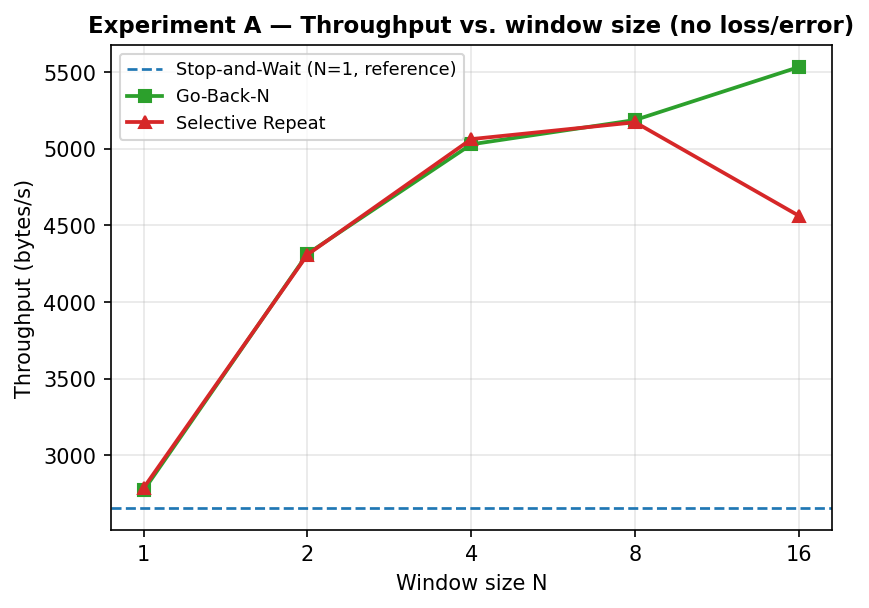
\includegraphics[width=0.85\textwidth]{figures/exp_a_throughput.png}
\caption{Throughput vs. window size $N$, no loss/error.}
\end{figure}
\begin{figure}[H]
\centering
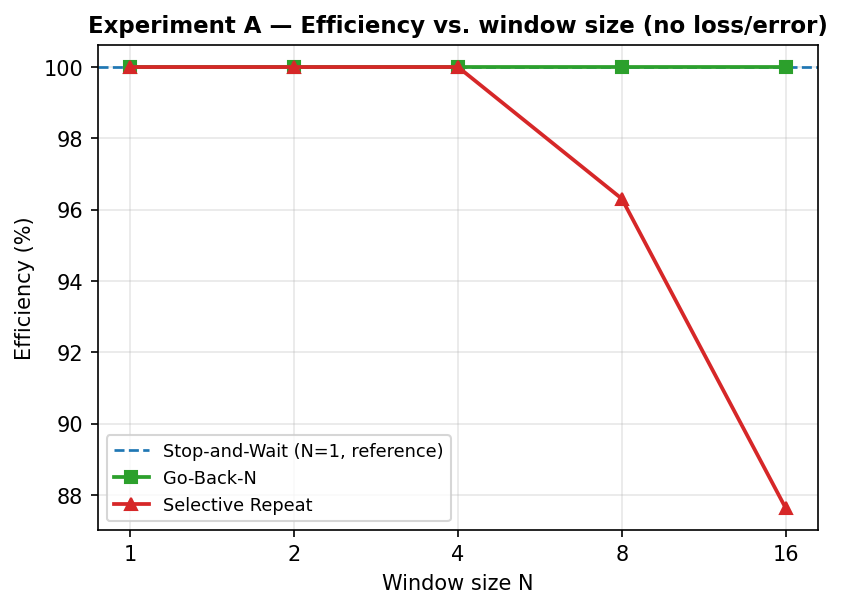
\includegraphics[width=0.85\textwidth]{figures/exp_a_efficiency.png}
\caption{Efficiency vs. window size $N$, no loss/error.}
\end{figure}
\begin{figure}[H]
\centering
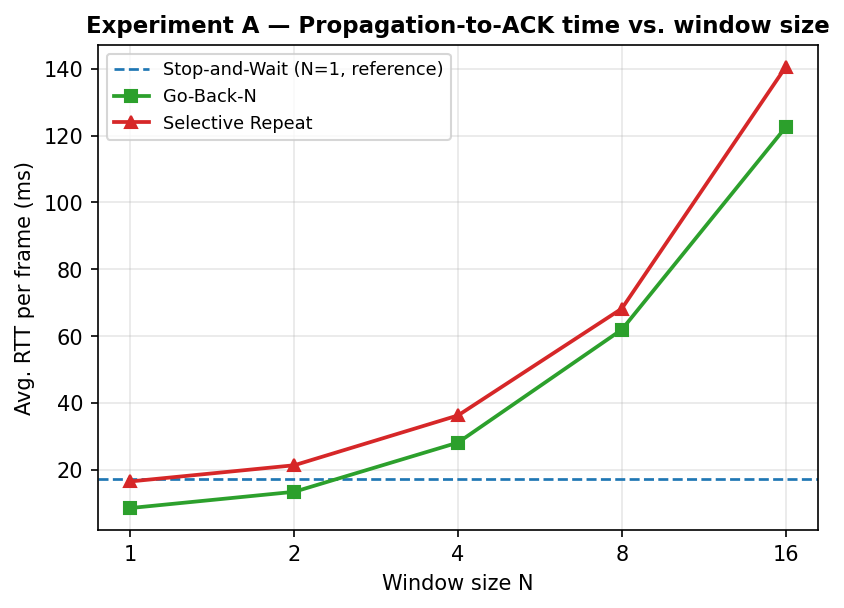
\includegraphics[width=0.85\textwidth]{figures/exp_a_rtt.png}
\caption{Average propagation-to-ACK time (RTT) vs. window size $N$.}
\end{figure}

\subsection{Experiment B --- Efficiency vs. Channel Impairment Probability}
A 66-frame file was transferred with Go-Back-N/Selective Repeat fixed at $N=4$, sweeping
the combined impairment probability $p \in \{0, 0.1, \dots, 0.5\}$
($\text{lossProb} = \text{errorProb} = p/2$, applied to both the data and ACK channels).

\begin{table}[H]
\centering
\small
\begin{tabular}{lrrrrr}
\toprule
\textbf{Protocol} & \textbf{p} & \textbf{Retransmissions} & \textbf{Elapsed (ms)} & \textbf{Throughput (B/s)} & \textbf{Efficiency (\%)} \\
\midrule
Stop-and-Wait & 0.0 & 0   & 1029.96 & 2912.75 & 100.00 \\
Stop-and-Wait & 0.1 & 11  & 1531.50 & 1958.87 & 85.71 \\
Stop-and-Wait & 0.2 & 48  & 3169.43 & 946.54  & 57.90 \\
Stop-and-Wait & 0.3 & 43  & 2793.23 & 1074.03 & 60.55 \\
Stop-and-Wait & 0.4 & 95  & 5059.14 & 592.99  & 40.99 \\
Stop-and-Wait & 0.5 & 141 & 8094.96 & 370.60  & 31.88 \\
\midrule
Go-Back-N ($N{=}4$) & 0.0 & 0   & 634.60  & 4727.42 & 100.00 \\
Go-Back-N ($N{=}4$) & 0.1 & 32  & 1413.03 & 2123.10 & 67.35 \\
Go-Back-N ($N{=}4$) & 0.2 & 63  & 2088.72 & 1436.29 & 51.16 \\
Go-Back-N ($N{=}4$) & 0.3 & 121 & 4379.94 & 684.94  & 35.29 \\
Go-Back-N ($N{=}4$) & 0.4 & 244 & 7068.33 & 424.43  & 21.29 \\
Go-Back-N ($N{=}4$) & 0.5 & 225 & 9253.55 & 324.20  & 22.68 \\
\midrule
Selective Repeat ($N{=}4$) & 0.0 & 0   & 565.70  & 5303.13 & 100.00 \\
Selective Repeat ($N{=}4$) & 0.1 & 14  & 1318.66 & 2275.04 & 82.50 \\
Selective Repeat ($N{=}4$) & 0.2 & 27  & 2062.62 & 1454.46 & 70.97 \\
Selective Repeat ($N{=}4$) & 0.3 & 58  & 2406.41 & 1246.67 & 53.23 \\
Selective Repeat ($N{=}4$) & 0.4 & 84  & 5955.47 & 503.74  & 44.00 \\
Selective Repeat ($N{=}4$) & 0.5 & 139 & 7248.13 & 413.90  & 32.20 \\
\bottomrule
\end{tabular}
\caption{Experiment B: efficiency/throughput vs. combined channel impairment probability
$p$, 66 frames, CRC-32.}
\label{tab:expB}
\end{table}

\begin{figure}[H]
\centering
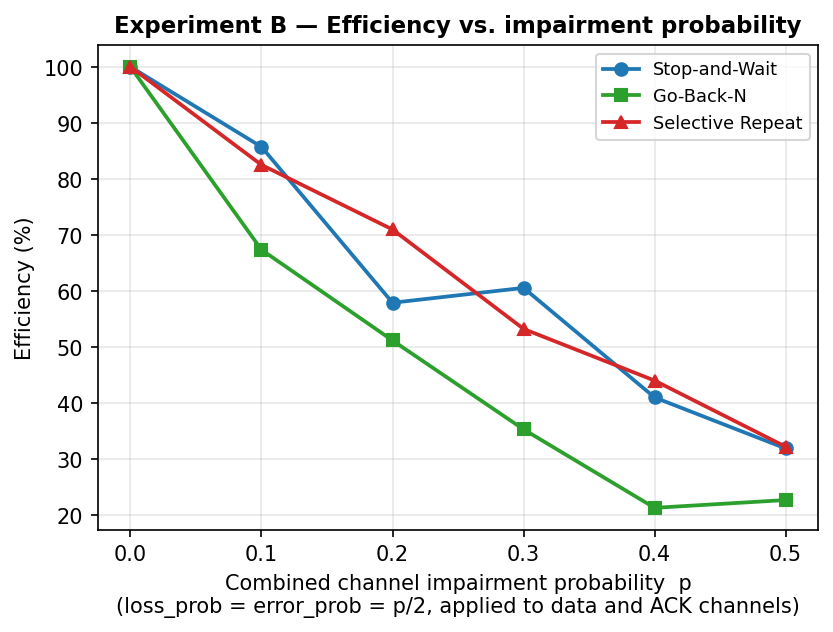
\includegraphics[width=0.85\textwidth]{figures/exp_b_efficiency.png}
\caption{Efficiency vs. impairment probability $p$.}
\end{figure}
\begin{figure}[H]
\centering
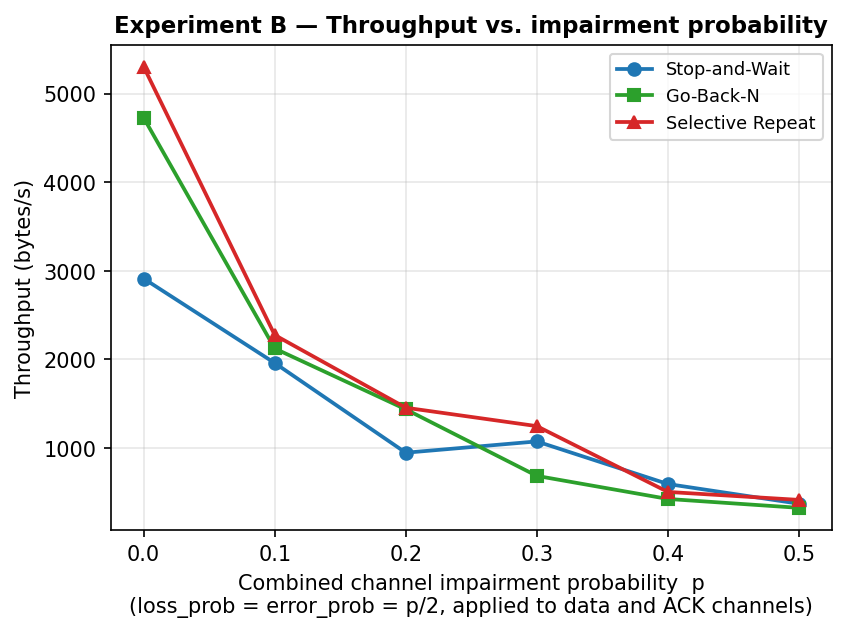
\includegraphics[width=0.85\textwidth]{figures/exp_b_throughput.png}
\caption{Throughput vs. impairment probability $p$.}
\end{figure}
\begin{figure}[H]
\centering
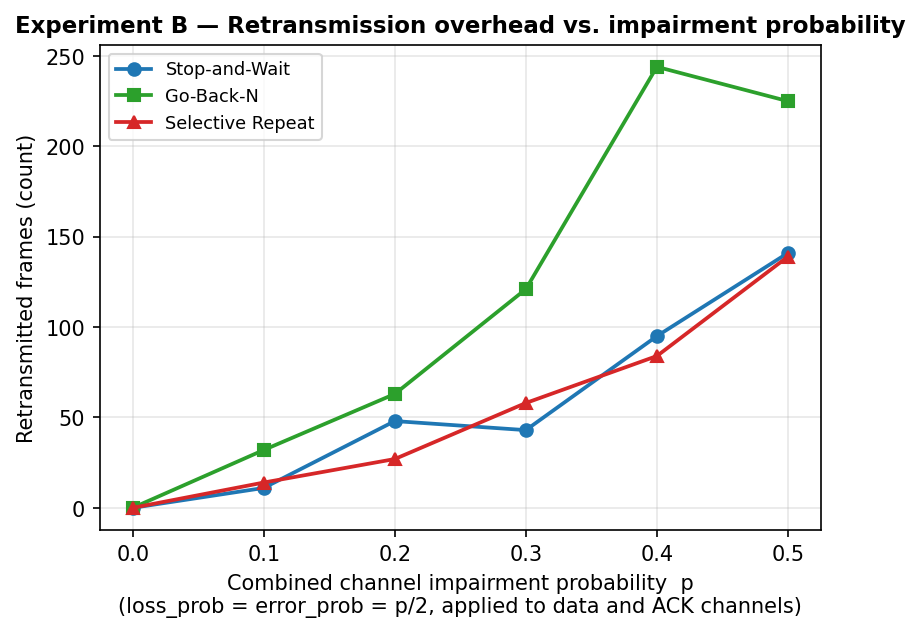
\includegraphics[width=0.85\textwidth]{figures/exp_b_retransmissions.png}
\caption{Retransmitted-frame count vs. impairment probability $p$.}
\end{figure}

\section{Analysis}

\paragraph{Windowing gain on a clean channel (Table~\ref{tab:expA}).} Stop-and-Wait can
only ever have one frame outstanding, so total time $\approx \text{frames} \times
\text{RTT}_{\text{frame}}$ — $730 \times 17.3\,\text{ms} \approx 12.6\,\text{s}$, exactly
what was measured. Go-Back-N/Selective Repeat need only $\lceil \text{frames}/N \rceil$
round trips instead of \text{frames}, because $N$ frames go out back-to-back before the
sender must wait; average RTT grows with $N$ (a larger batch takes longer to be fully
ACKed) but not proportionally to $N$, since the simulated channel only adds 1--15\,ms of
random delay per frame — so wall-clock time keeps falling and throughput keeps climbing,
roughly doubling from $N{=}1$ to $N{=}4$ and again by $N{=}16$, with diminishing returns
past $N{=}8$ as loopback/processing overhead rather than RTT becomes the bottleneck.

\paragraph{Selective Repeat's efficiency dip at large $N$, zero configured loss.} At
$N{=}8$ and $N{=}16$, Selective Repeat's efficiency falls to 96.3\% and 87.6\% respectively
even though \texttt{lossProb} $=$ \texttt{errorProb} $=0$ — every one of those
``retransmissions'' is spurious. Selective Repeat computes each frame's deadline at send
time from the \emph{current} adaptive timeout estimate; when a large batch of $N$ frames is
sent, the later frames in that batch are naturally ACKed later than the earlier ones, but
the estimator (still centered on a smaller-window RTT from earlier in the transfer) has not
yet ``learned'' the larger batch's true round-trip time. A tail frame can therefore miss its
deadline and be resent even though nothing was actually lost — and because Karn's rule
excludes retransmitted samples from updating the estimator, the correction is slow. Go-Back-N
did not exhibit this in these runs because it uses one shared timer keyed to the
\emph{oldest} outstanding frame rather than $N$ independent per-frame deadlines, which is
coarser and less prone to spurious firing; this is a genuine per-protocol timer-design
trade-off rather than a bug, and it is worth noting that Experiment A used a single run per
configuration, so some of the difference between Go-Back-N and Selective Repeat here may
also reflect run-to-run variance rather than a strict rule.

\paragraph{Efficiency and throughput under increasing impairment (Table~\ref{tab:expB}).}
All three protocols degrade monotonically as $p$ rises from 0 to 0.5, which follows directly
from $\text{efficiency} = \text{unique frames} / \text{frame transmissions}$: every loss or
corruption event forces at least one retransmission. The protocols separate clearly on
\emph{how much} one such event costs:
\begin{itemize}[leftmargin=1.6em]
  \item \textbf{Go-Back-N degrades worst} (225 retransmissions and 324\,B/s throughput at
  $p=0.5$, versus 141/371\,B/s for Stop-and-Wait and 139/414\,B/s for Selective Repeat).
  A single lost/corrupted data frame \emph{or} ACK anywhere within the window of $N{=}4$
  forces the \emph{entire} window to be retransmitted, so its retransmission cost scales
  with $N$ — the textbook weakness of Go-Back-N under a lossy channel.
  \item \textbf{Selective Repeat tracks Stop-and-Wait closely} despite pipelining, because
  it only ever retransmits the specific frame that actually failed — its ``waste
  multiplier'' stays at 1$\times$ regardless of $N$, identical to Stop-and-Wait. This is
  exactly Selective Repeat's textbook motivation: Go-Back-N's throughput on a clean channel
  without Go-Back-N's retransmission tax when the channel is lossy. At $p=0.5$ it delivers
  higher throughput than Stop-and-Wait (413.9 vs.\ 370.6\,B/s) for essentially the same
  retransmission cost.
\end{itemize}

\paragraph{Why average RTT stays flat (15--37\,ms) across all $p$ (not shown by protocol in
the RTT columns of Table~\ref{tab:expB}, but confirmed in the raw logs) while elapsed time
and efficiency clearly do not.} Karn's algorithm explicitly excludes retransmitted frames
from RTT sampling, so \texttt{avg\_rtt\_ms} only ever measures genuinely successful
first-attempt round trips — a proxy for pure channel propagation/processing delay,
deliberately insensitive to loss probability. This is also a useful correctness check: if
the RTT estimator were (incorrectly) sampling retransmitted frames, it would drift upward
with $p$, which it does not.

\paragraph{A non-monotonic data point worth flagging.} Go-Back-N's efficiency ticks up
slightly from $p{=}0.4$ to $p{=}0.5$ (21.29\% $\to$ 22.68\%) instead of continuing to fall.
This is not a real effect: each row in Table~\ref{tab:expB} is a \emph{single} run rather
than an average over several trials, so the random channel draws at one probability can
happen to align better or worse than at a neighbouring probability. Averaging 3--5 runs per
configuration (or using a longer input file) would smooth this out; it is noted here rather
than hidden.

\subsection{Known Bugs Found and Fixed During Testing}
Two real defects were caught by the end-to-end \texttt{diff} check (not merely by
compiling) and are recorded here for completeness rather than smoothed over:
\begin{enumerate}[leftmargin=1.6em]
  \item \textbf{Duplicate-datagram misparse crash.} The original \texttt{SETUP} handshake
  sent three redundant copies of the 8-byte setup datagram; the receiver's
  \texttt{recvSetup()} consumed only the first, leaving the other two sitting in the
  socket's receive queue. The main receive loop then occasionally read one of those 8-byte
  datagrams and passed it to \texttt{DataFrame::fromBytes()}, which indexed past the end of
  an 8-byte buffer expecting 65 bytes and crashed with \texttt{std::out\_of\_range}. Fixed
  by sending \texttt{SETUP} exactly once (loopback UDP between two local processes is an
  in-kernel copy and does not drop) and by adding an explicit datagram-size check before
  parsing on every receive path (TC9).
  \item \textbf{Sender/receiver livelock on a lost final ACK.} If the very last ACK of a
  transfer was itself dropped by the simulated channel, the sender would retransmit
  indefinitely into a receiver process that had already delivered every frame and exited,
  hanging the whole run. Fixed with a bounded grace period on the receiver side after the
  last frame is delivered, so it stays alive just long enough to re-ACK a late retransmission
  before exiting.
\end{enumerate}

\section{Comments}

\paragraph{Evaluation of the Lab Assignment.} This assignment moved the focus from
single-frame integrity (Assignment 1) to multi-frame session reliability, which is a
qualitatively different engineering problem: correctness now depends on timing (when does a
retransmission fire), not just on data (is this frame's FCS valid). Building three
protocols side by side on one shared channel simulation made the textbook trade-offs
(Stop-and-Wait's idle time, Go-Back-N's window-wide retransmission cost, Selective Repeat's
buffering requirement) directly measurable rather than only theoretical.

\paragraph{Difficulty and Learning Outcomes.} The hardest part was not any single
protocol's happy path but getting the \emph{failure} paths right: Karn's algorithm for RTT
sampling, the exact receive-window arithmetic for Selective Repeat's ``previous window''
duplicate case, and the two livelock/crash bugs in \S5.3, both of which only appeared under
sustained loss and would have been invisible without an automated, high-iteration test
harness. Implementing the adaptive timer also made concrete why a fixed timeout is a poor
choice: at $N{=}16$ in Experiment A the true RTT was over $7\times$ the $N{=}1$ RTT, and a
timeout tuned for one would either fire constantly at the other or recover far too slowly.

\paragraph{Suggested Improvements.} Averaging multiple trials per configuration (flagged
explicitly in \S4) would remove the single-run noise visible in Table~\ref{tab:expB} and
make the efficiency curves strictly monotonic. Selective Repeat's spurious-timeout behavior
at large $N$ (\S4) could also be reduced by seeding each frame's initial deadline from a
window-size-aware estimate rather than the same shared estimator Stop-and-Wait uses, which
would be a natural follow-up experiment.

\end{document}
